\myslide{Outline}
{
  \begin{itemgroup}{"Ubersicht}
    \item Ausdr"ucke und Typen k"onnen in ihrer Baumansicht betrachtet werden
    \item Schwierige Ausdr"ucke k"onnen so besser verstanden werden
    \item Name der Ausd"ucke und Typen wird dargestellt
    \item Menge der Ausdr"ucke und Typen wird dargestellt
    \item Der Index wird ebenfalls eingeblendet
    \item Bindungen von Identifiern k"onnen betrachtet werden
    \item Die Outline muss bei neuen Ausdr"ucken nicht angepasst werden,
          sondern "ubernimmt diese automatisch
  \end{itemgroup}
}

\myslide{Outline}
{
  \begin{itemgroup}{Einstellungen}
    \item \glqq Hervorheben\grqq: Selektierte Knoten werden in h"oheren Knoten markiert
    \item \glqq Gebundene\grqq: Gebundene Identifier werden markiert
    \item \glqq Freie\grqq: Frei vorkommende Identifier werden markiert
    \item \glqq Ersetzen\grqq: Selektierte Knoten werden durch \glqq ...\grqq\ ersetzt
    \item \glqq Source Code\grqq: Der zu dem selektierten Knoten passende Source Code
                                  wird im Editor hervorgehoben
    \item \glqq Auto Update\grqq: Die Outline wird bei "Anderungen automatisch aktualisiert
  \end{itemgroup}
}

\myslide{Outline}
{
  \begin{center}
    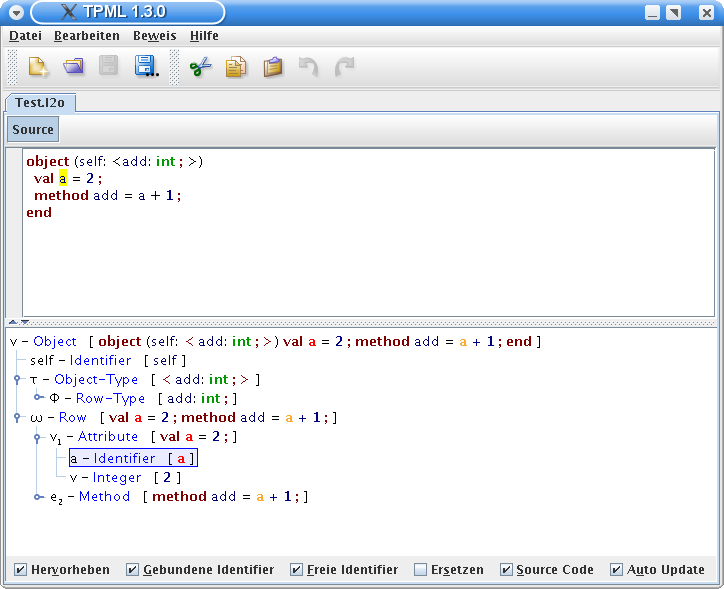
\includegraphics[height=15cm]{images/outline.png}
  \end{center}
}